\documentclass{article}
\usepackage{xspace}
\usepackage{graphicx}

\title{Technical report for Workshop 1.5 data analysis}
\author{S.~Sinclair}

\newcommand{\emerge}{\textsc{[E]merge}\xspace}
\newcommand{\todo}[1]{\emph{To do: #1}}

\begin{document}
\maketitle

\begin{abstract}
This document presents a summary of analysis techniques used to
interpret the data collected during the \emerge ``Workshop 1.5''
recording session, which took place Apr. 30, 2011.
\end{abstract}

\section{Overview}

\todo{Description of data collection (data format, metadata, time handling, etc.)}

10 Hz, range 10 bit.  8 minibees were recorded.  Current video frame,
time of data reception was recorded.  Video was tagged manually
afterwards.

\todo{Overview of analysis approach (features, prediction)}

\todo{List of features}

\begin{itemize}
  \item Amplitude (root mean square).
  \item Frequency and periodicity.
    \begin{itemize}
    \item Zero-crossing analysis.
    \item Autocorrelation.
    \end{itemize}
  \item Visualized range/variance---analysis of linear regression
    angle and variance in plots of data.
  \item Covariance/correlation analysis.
  \item Max/min over various window sizes.
  \item Jerk.
\end{itemize}

\todo{Comparison methods}

\begin{itemize}
  \item Neural net prediction performance
\end{itemize}

\section{Features}

\subsection{Amplitude (root mean square)}

Anyone.

\subsection{Frequency and periodicity}

\subsubsection{Zero-crossing analysis}

(Steve)

\subsubsection{Autocorrelation}

(Steve)

\subsection{Visualized range/variance}

Plotting linear regression angle and deviation size. (Joe)

\subsection{Covariance/correlation analysis}

(Joe/Steve)

\subsection{Max/min over various window sizes}

(Sofian)

\subsection{Jerk}

(Sofian)

\section{Comparison methods}

\subsection{Neural net prediction}

Fig.~\ref{fig:predresults} shows error in the prediction using RMS and
zero-crossing-derived frequency and periodicity.

(Steve)

\begin{figure}
\centerline{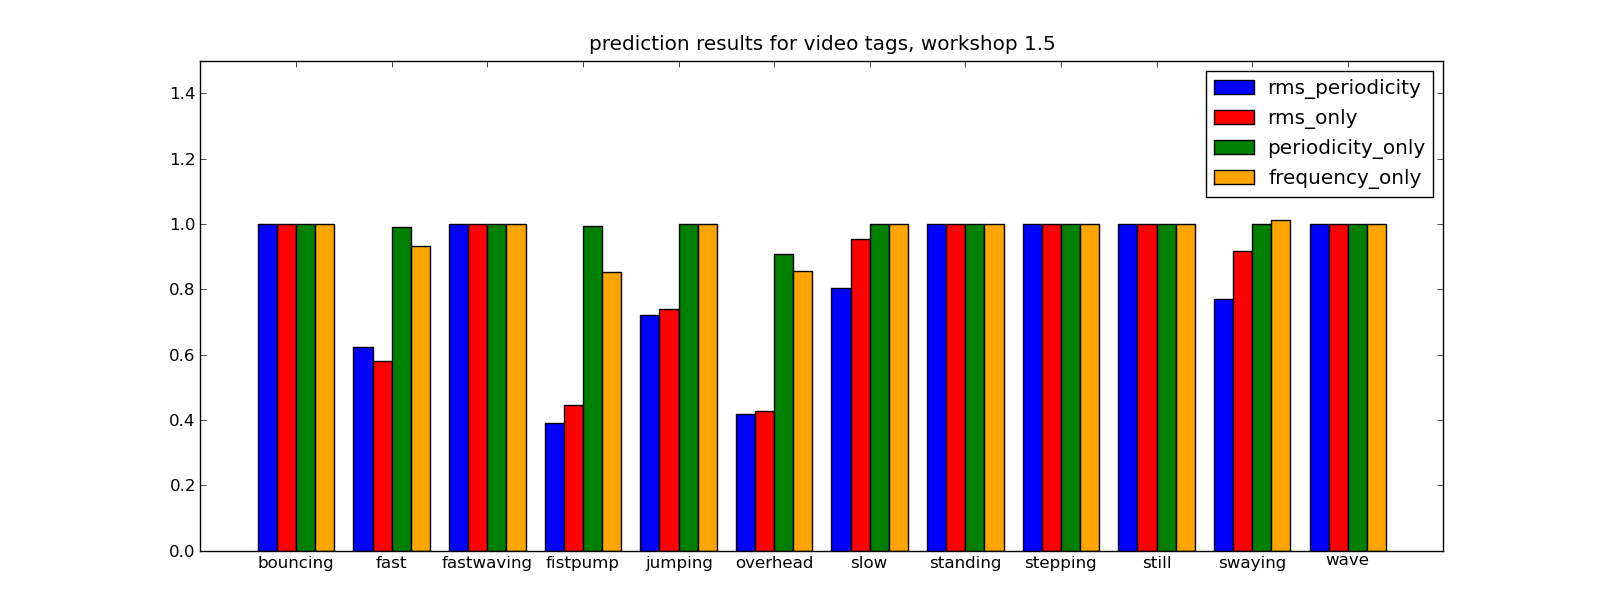
\includegraphics[width=\textwidth]{images/predictionresults.png}}
\caption{Ability of RMS, zero-crossing periodicity and frequency
  features to predict the video tags.  1 indicates 100\% error, zero
  indicates no error.  It can be seen that RMS seems to basically just
  predict activity; periodicity and frequency are not contributing.}
\label{fig:predresults}
\end{figure}

\end{document}
